\subsubsection[The \xtsvty]{The $\boldsymbol{\xtsvty}$}
\label{sec:x1070}

While searching for potential backgrounds resulting from misidentifying two hadrons as muons, a
peak was found in the invariant mass spectrum of the $K_\mu^+K_\mu^-$ candidates.
This peak was consistent with the \xtsvty listed in Ref.~\cite{PDG2014}, which has a mass of
$(1072\pm1)\mev$ with a width of $(3.5\pm0.5)\mev$ and was observed in the $\KS\KS$ distribution
from $\pim p \to \KS \KS n m\piz$ collisions~\cite{x1070vlad}, where $m\in\mathbb{Z}$.
Figure~\ref{fig:x1070} shows the observation of this resonance from \Ref{x1070vlad} alongside
the data from this analysis.

\begin{figure}
  \begin{center}
    %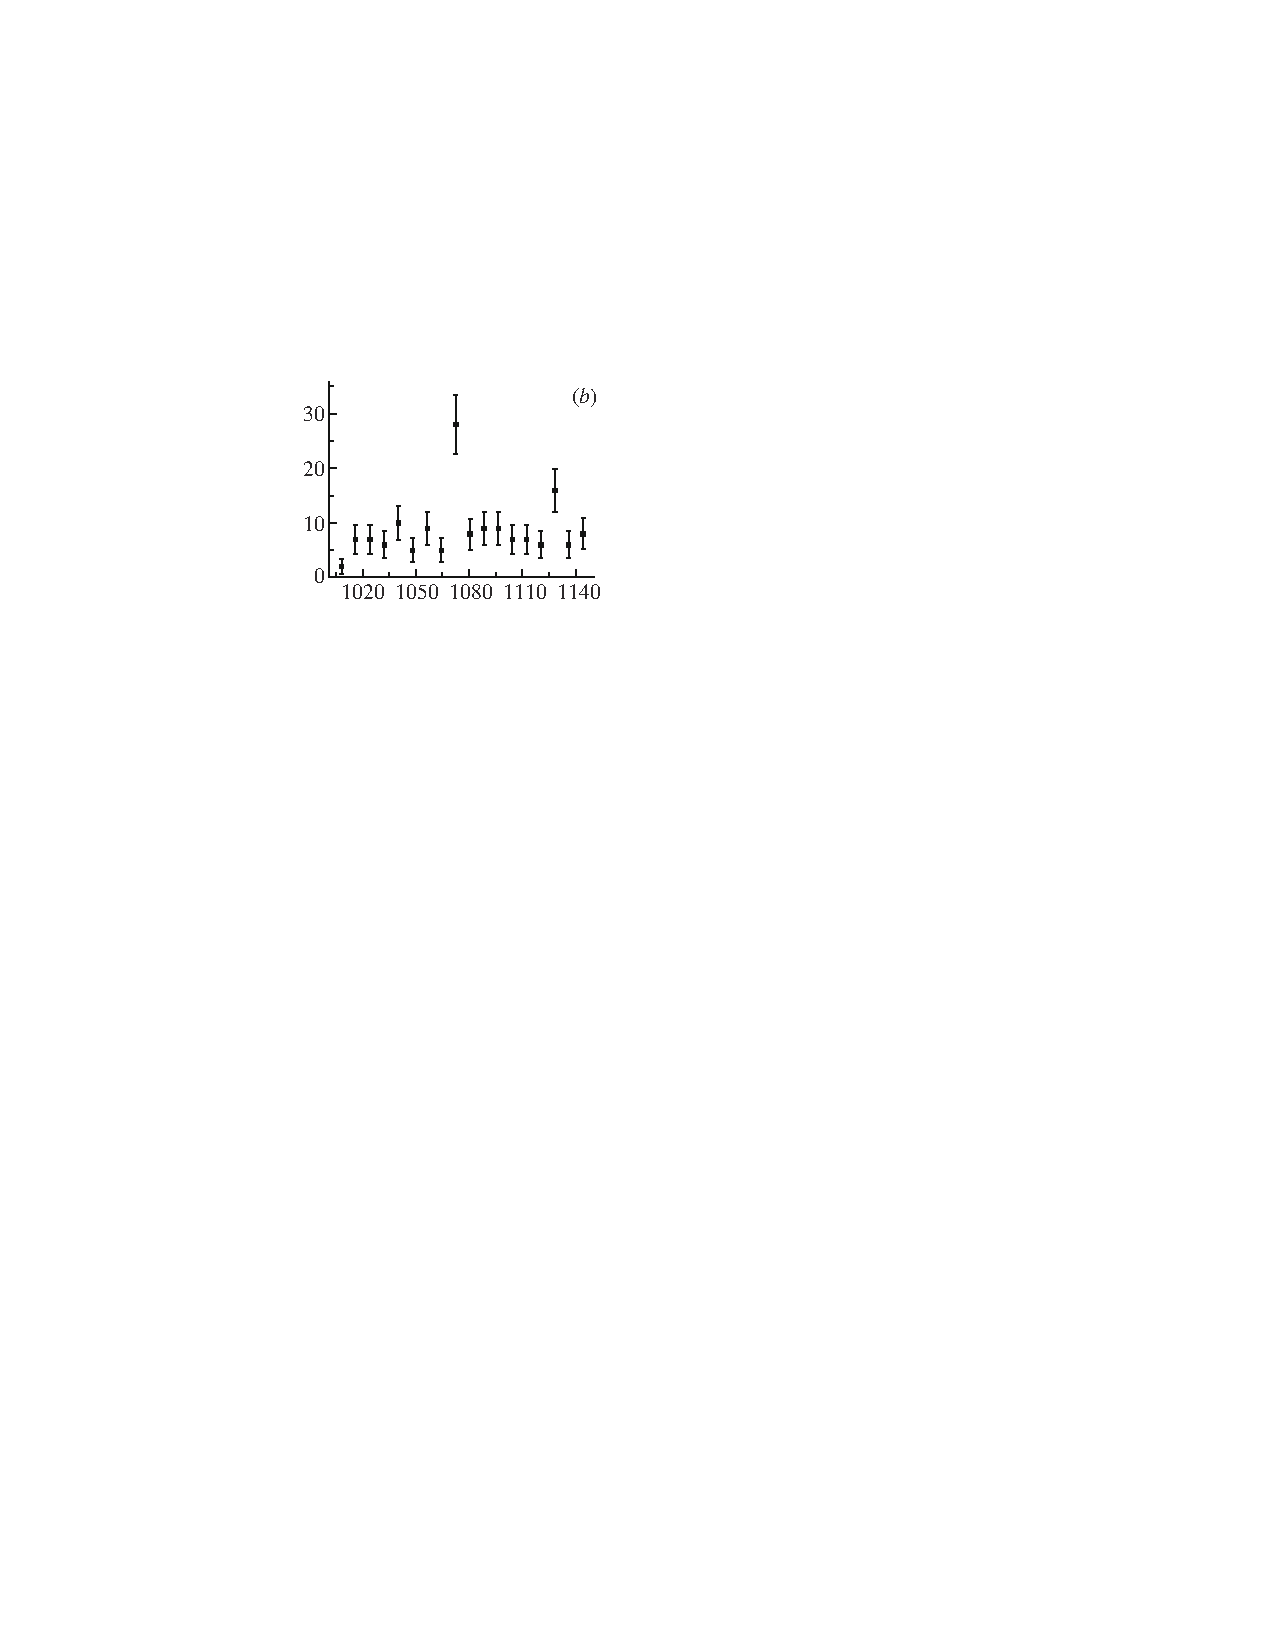
\includegraphics[height=0.2\textheight]{x1070vlad}
    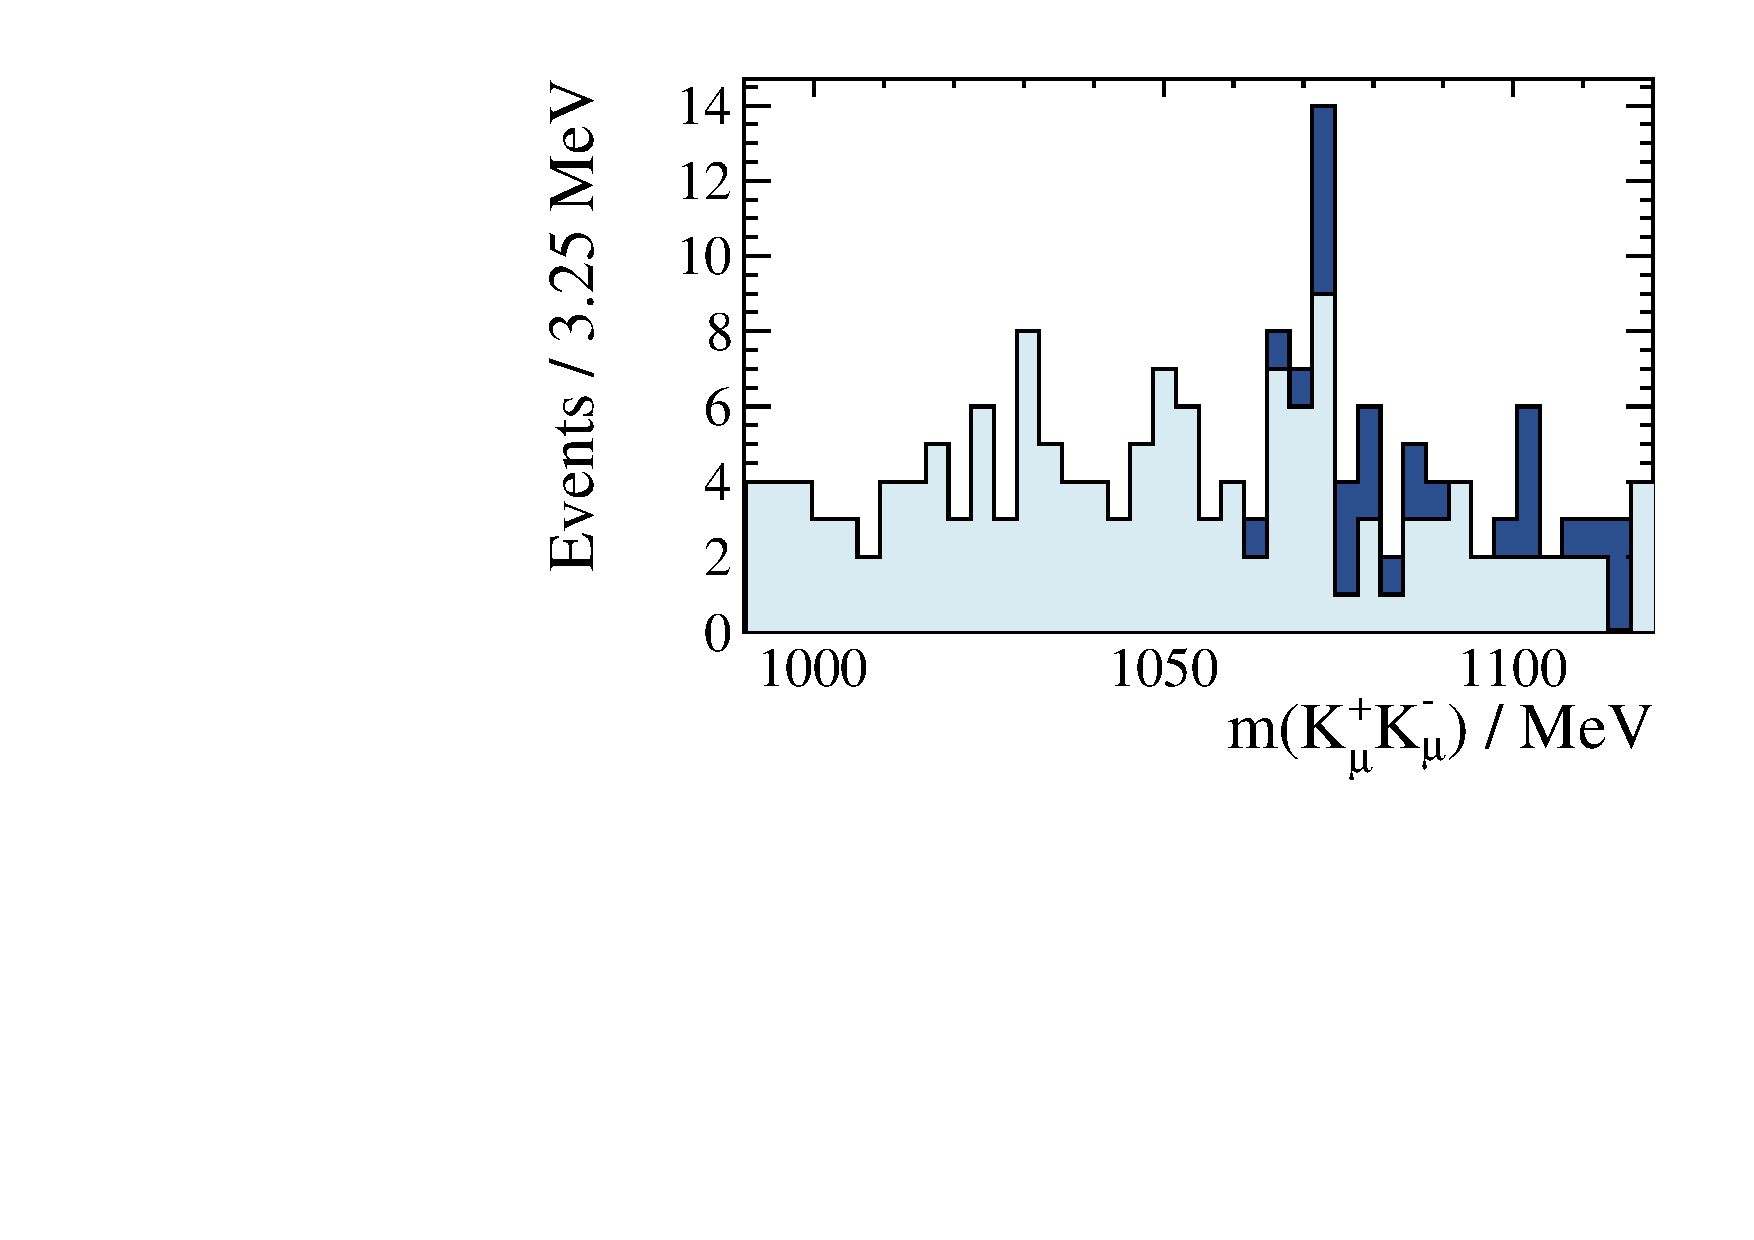
\includegraphics[height=0.2\textheight]{mumu_kk}
    \caption{
      %A comparison of
      %(left) the data which observes the \xtsvty~\protect\cite{x1070vlad}, and
      Invariant mass distribution of the $K_\mu^+K_\mu^-$ candidates in data, showing a peak at
      \approx$1072\mev$ in data.
      The dashed line indicates the effect of vetoing the decay
      \decay{\KS}{\pip\pim} in the preseletcion.
    }
    \label{fig:x1070}
  \end{center}
\end{figure}

Figure~\ref{fig:db:x1070:2d} shows a comparison of simulated \decay{\KS}{\pipi} decays with the
observed data near this excess.
It is clear that \decay{\KS}{\pipi} decays produce a peak around $1070\mev$ under the \kk
hypothesis.
There is also a long tail but with low statistics and with a roughly uniform
background this tail would not be expected to be visible in the data after the \KS veto in the
preselection.

\begin{figure}
  \begin{center}
    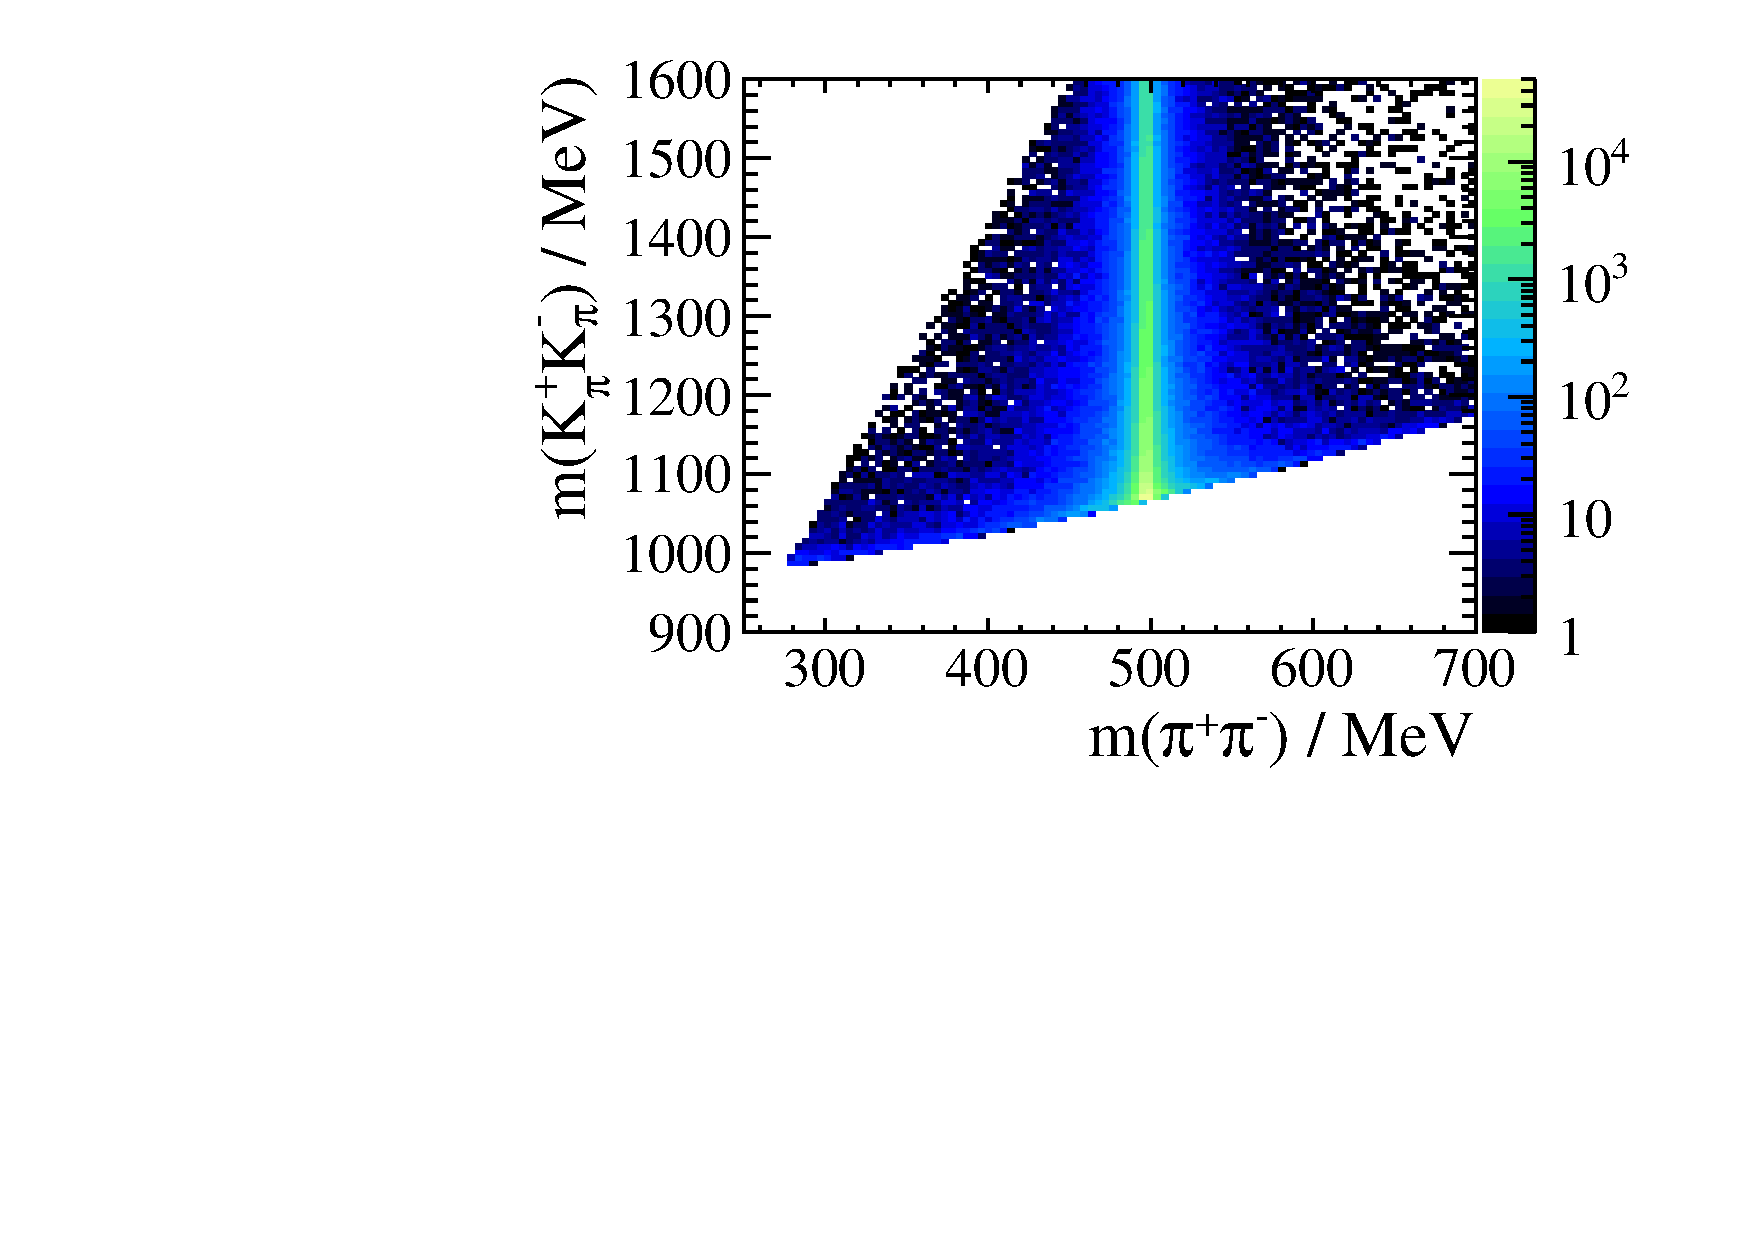
\includegraphics[width=0.48\textwidth]{gen_kk_pipi}
    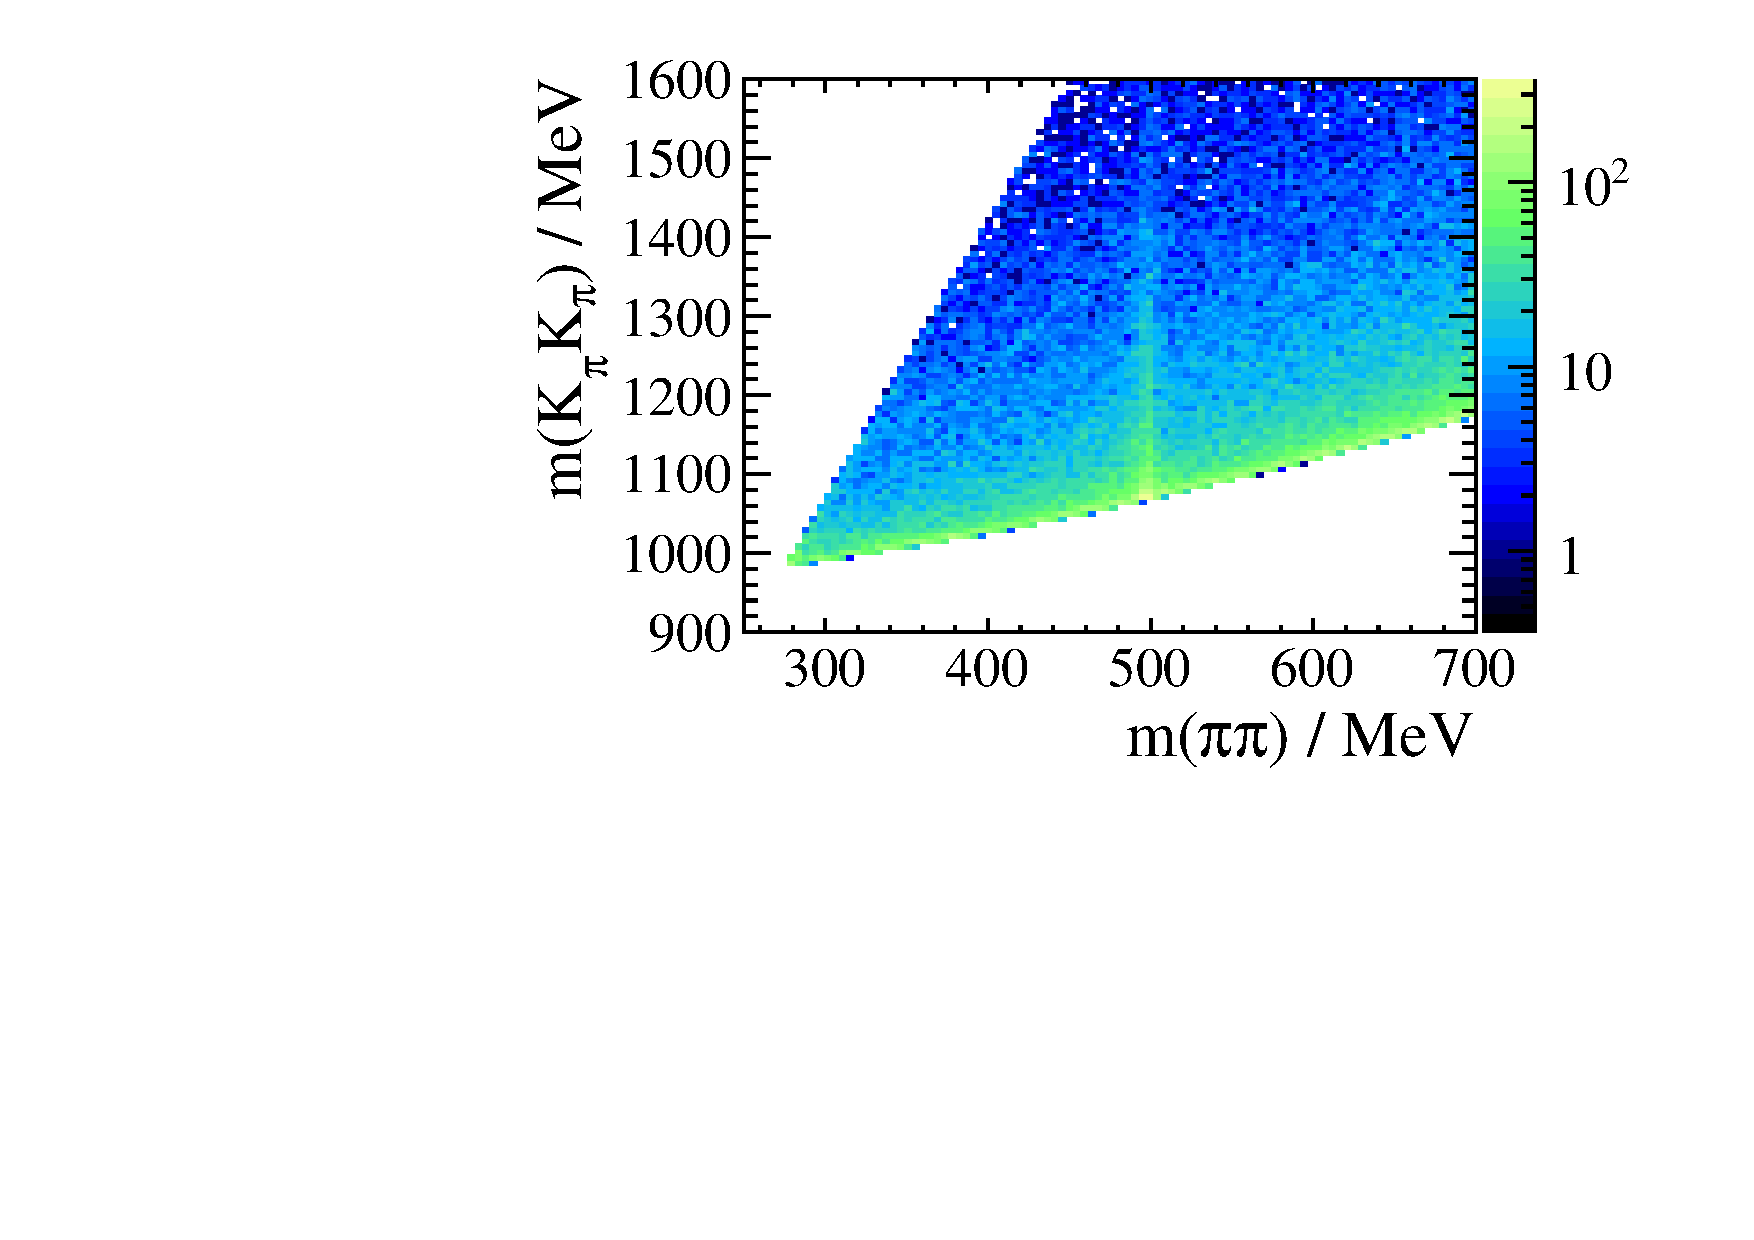
\includegraphics[width=0.48\textwidth]{data_kk_pipi}\\
    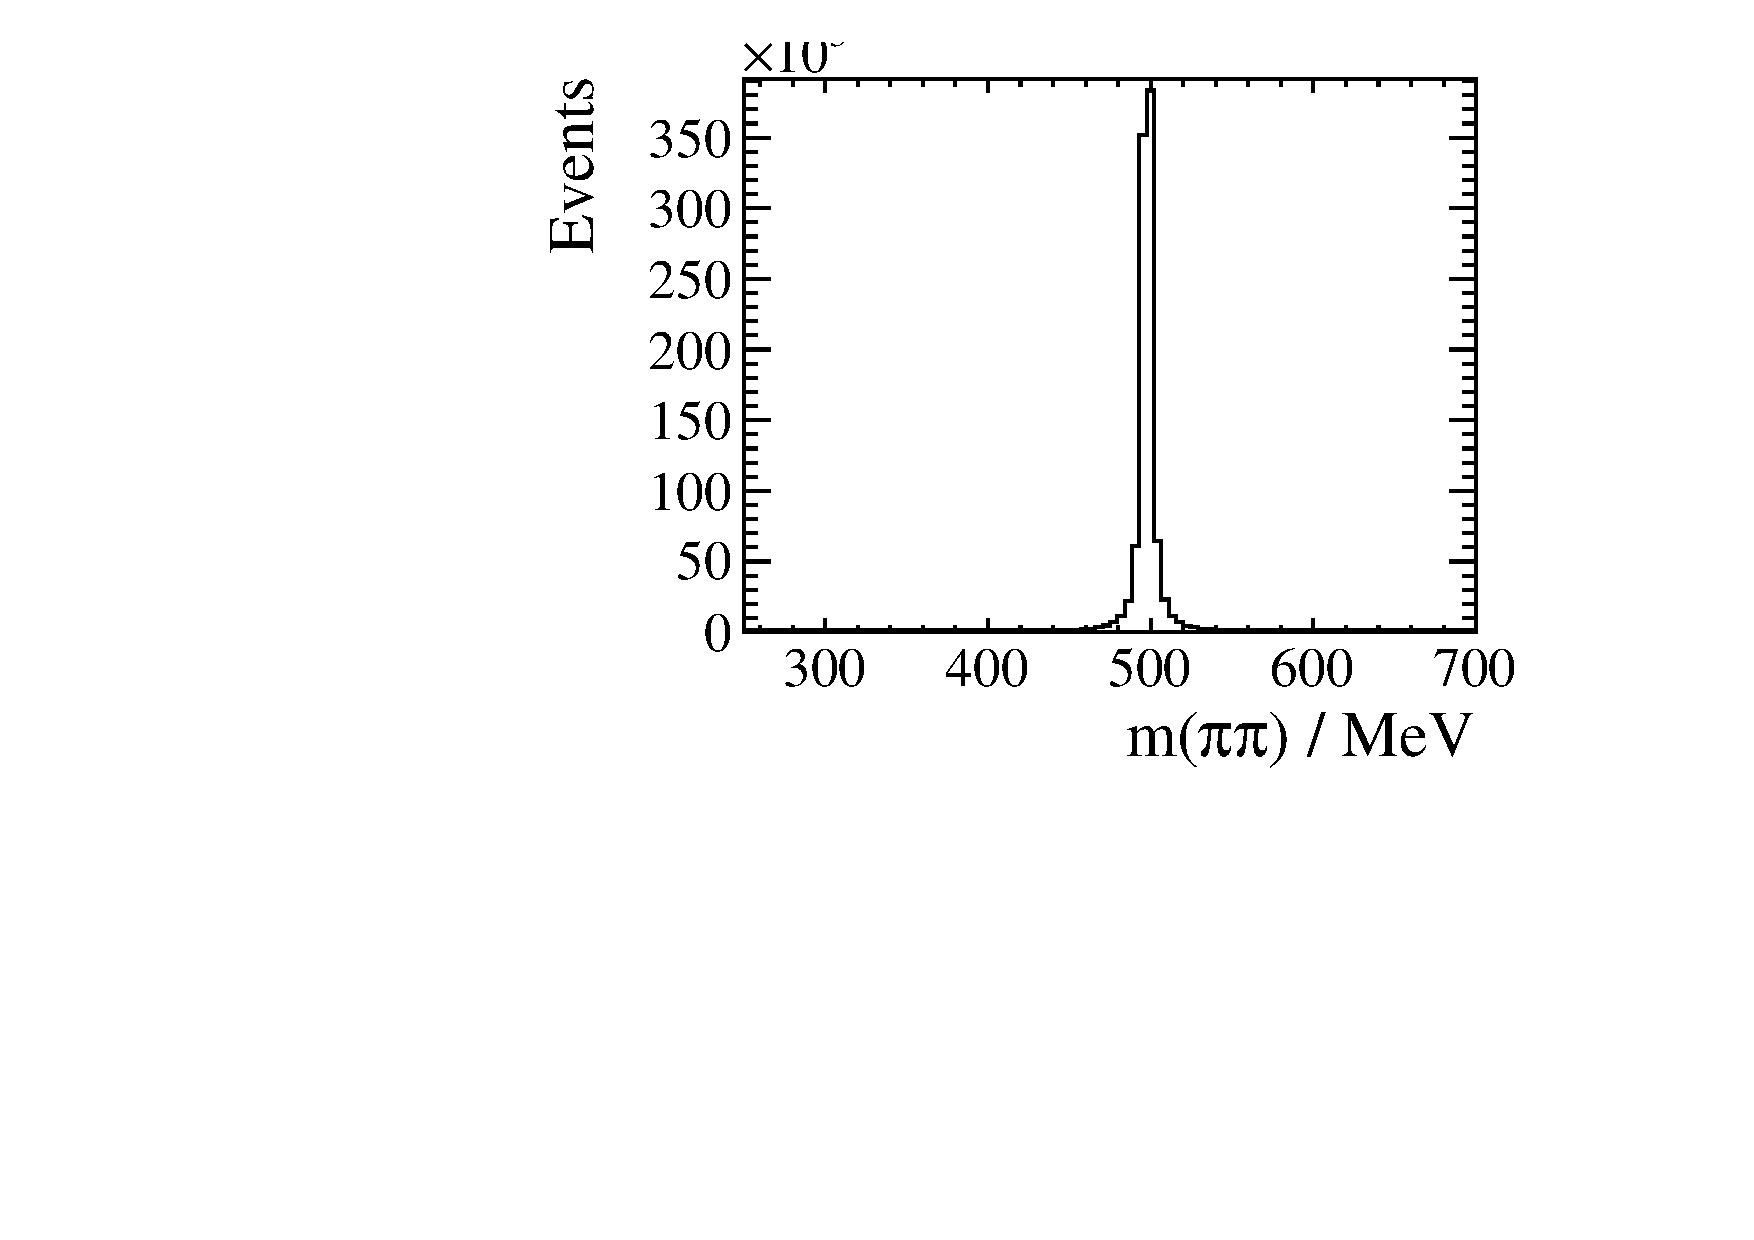
\includegraphics[width=0.48\textwidth]{gen_pipi}
    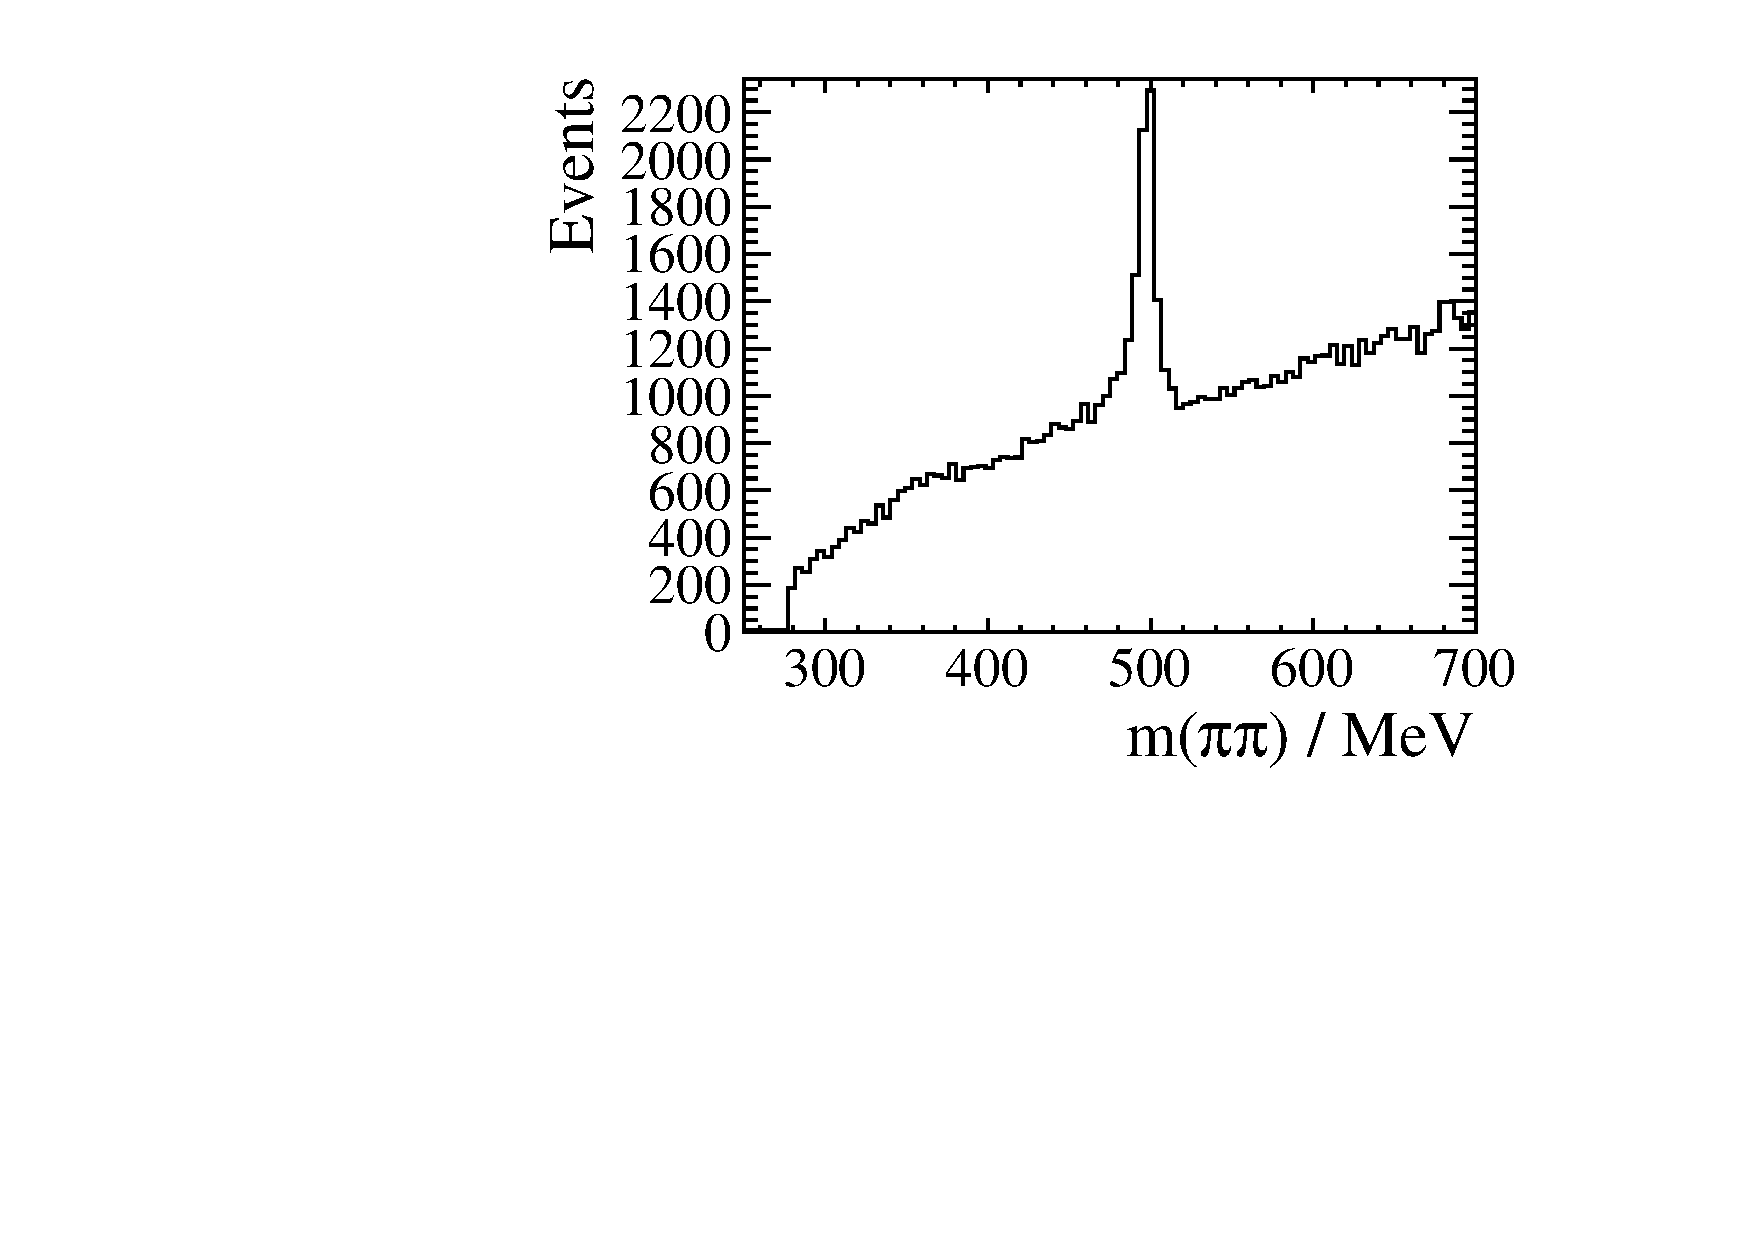
\includegraphics[width=0.48\textwidth]{data_pipi}\\
    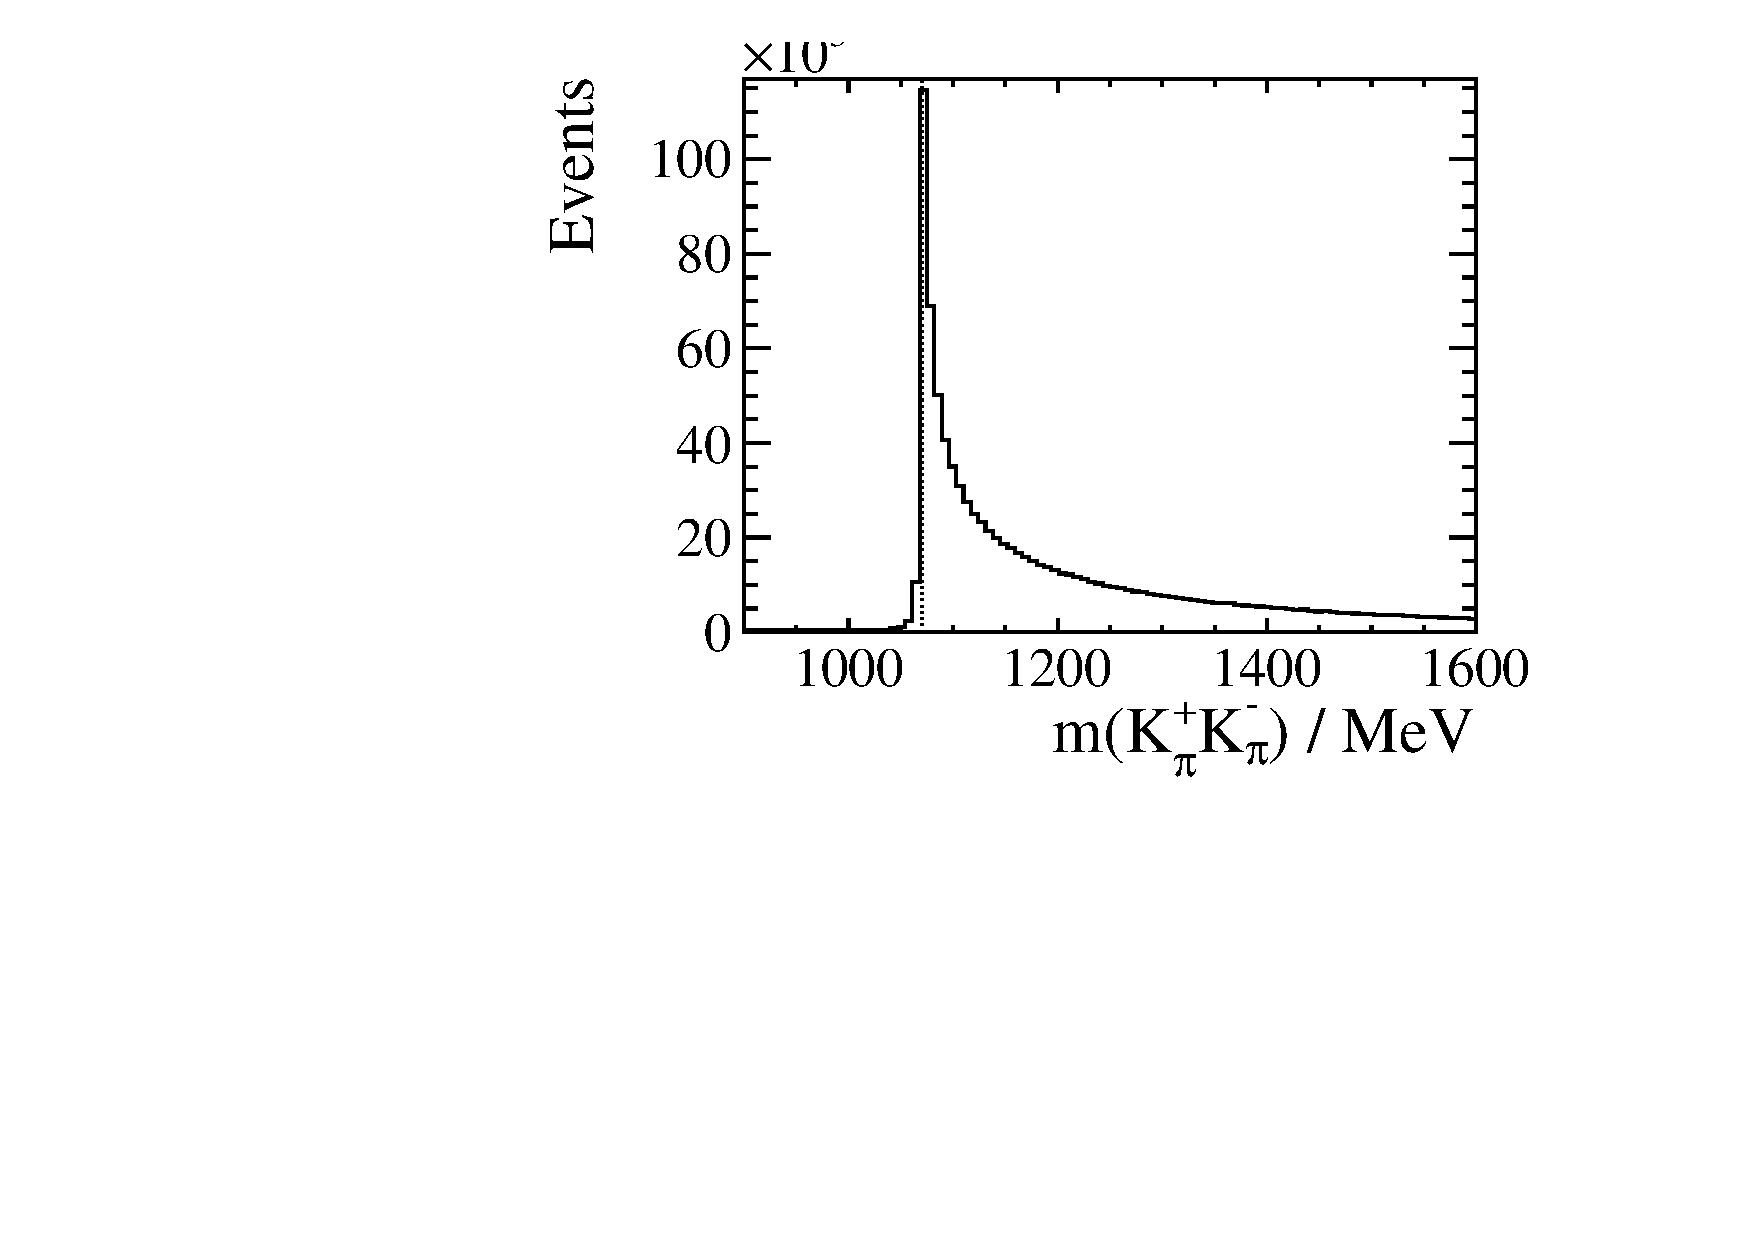
\includegraphics[width=0.48\textwidth]{gen_kk}
    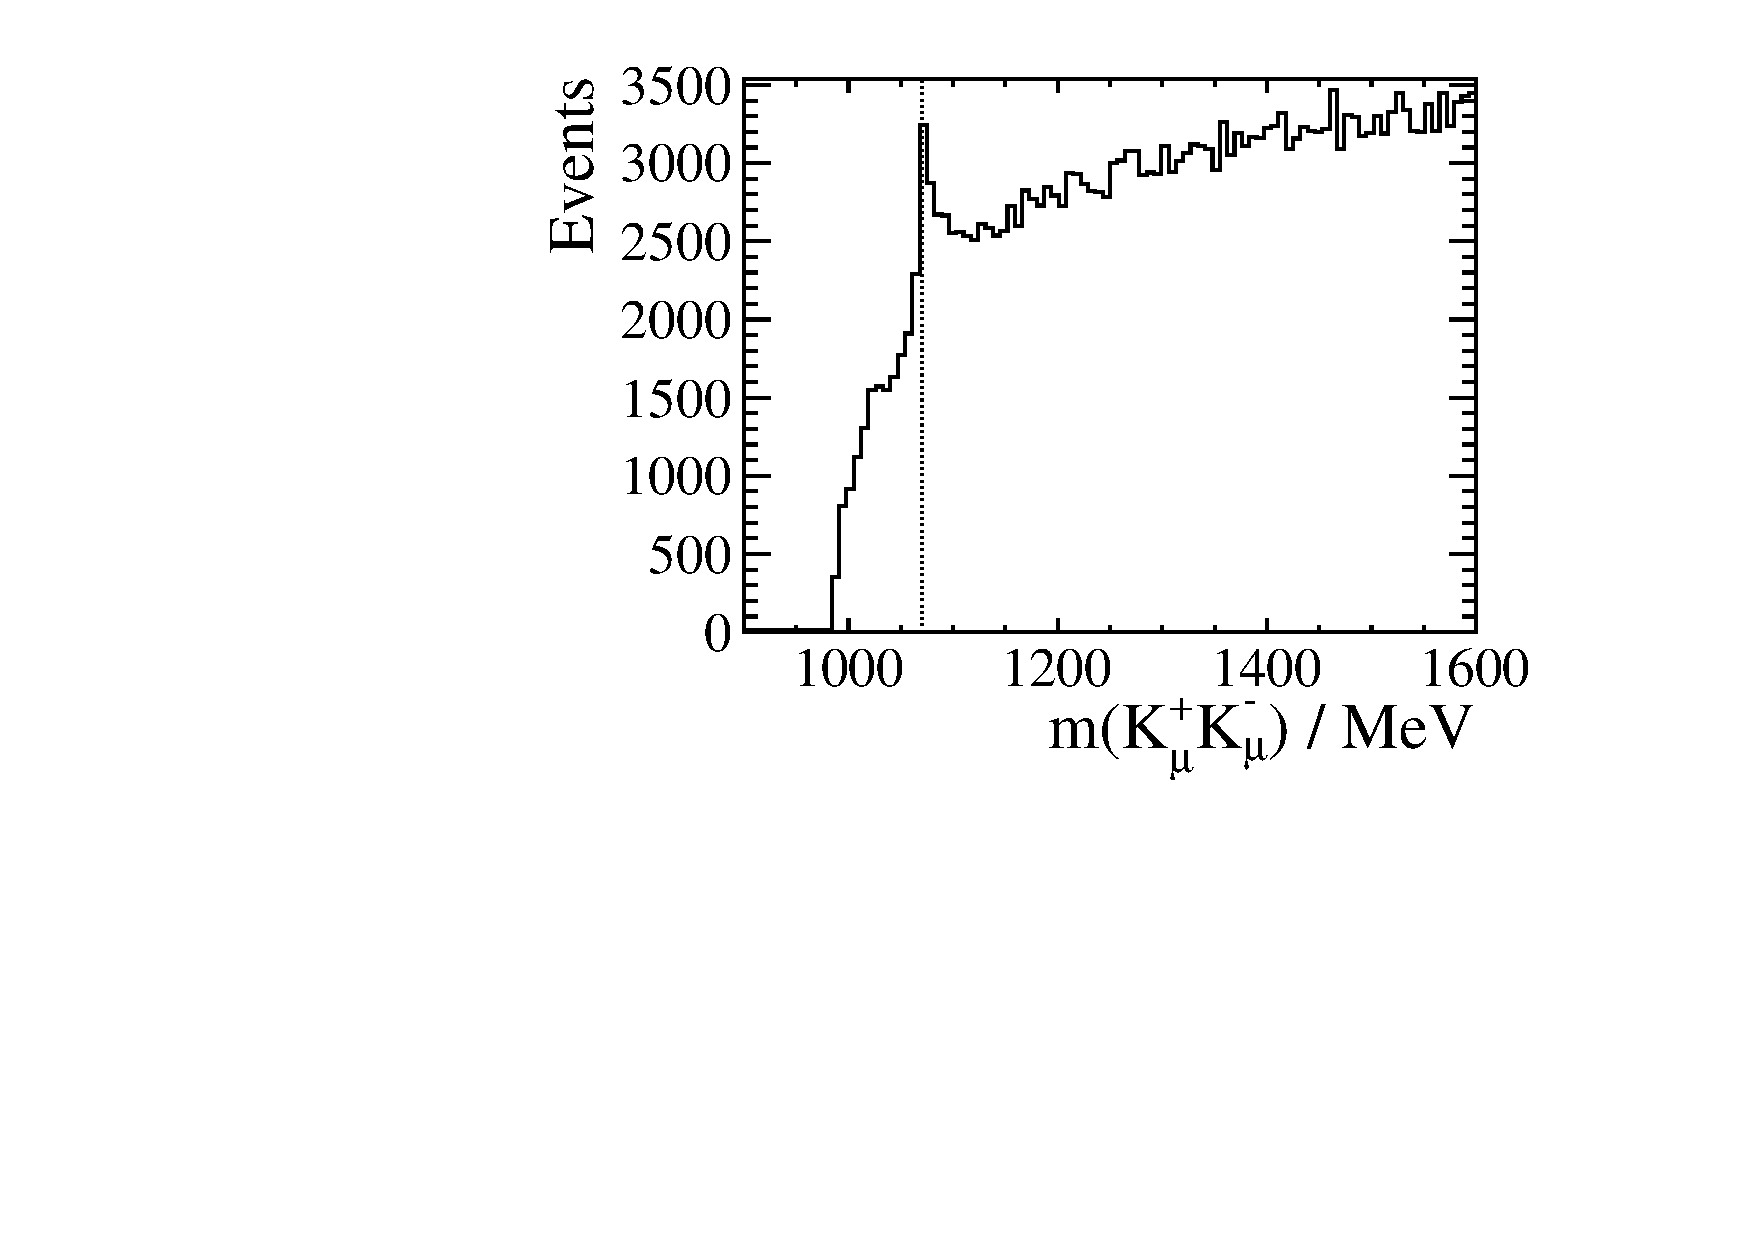
\includegraphics[width=0.48\textwidth]{data_kk}
    \caption{
      A comparison of \decay{\KS}{\pi\pi} under different mass hypotheses, for
      (left) simulated events, and
      (right) events from data.
      The (top) plots show the two dimensional distributions of the invariant mass distributions of
      a \pipi pair and the same candidates in the \kk mass hypothesis, the (middle) and (bottom)
      plots show the projections.
      Vertical lines in the lower plots indicate $1072\mev$.
    }
    \label{fig:db:x1070:2d}
  \end{center}
\end{figure}













